% =====================================================================
%  Midterm presentation — MA-INF 4330 Lab Explainable AI and Applications
%  "Finding the Safety Switches: Refusal Circuits Are Concentrated but Not Modular"
%  Pranav Yadav · University of Bonn
%
%  COMPILE WITH XeLaTeX (Exo 2 font via fontspec):
%      latexmk -xelatex -interaction=nonstopmode main.tex
%  Theme: github.com/fseiffarth/LatexBeamerThemeUniBonnStyle (vendored here).
% =====================================================================
\documentclass[aspectratio=169]{beamer}
\usepackage[T1]{fontenc}

\usetheme{UniBonn}

\usepackage{booktabs}
\usepackage{array}
\usepackage{tikz}
\usetikzlibrary{arrows.meta, positioning, fit, backgrounds}
\usepackage{pifont}                         % \ding check / cross marks

% --- verdict + accent helpers in the theme palette -------------------
\newcommand{\good}{\textcolor{themeblue!80!black}{\ding{51}}}
\newcommand{\bad}{\textcolor{red!70!black}{\ding{55}}}
\newcommand{\pmark}{\textcolor{themeorange!80!black}{$\sim$}}   % partial verdict
\newcommand{\hl}[1]{\textcolor{themeblue}{\textbf{#1}}}

% Theme uses \contour for the subitem bullet, which emits PS specials XeLaTeX's
% driver cannot interpret; replace with a plain themed dash.
\setbeamertemplate{itemize subitem}{\textcolor{themeblue}{--}}
\newcommand{\hlo}[1]{\textcolor{themeorange!75!black}{\textbf{#1}}}

% --- metadata --------------------------------------------------------
\title[Safety Switches]{Finding the Safety Switches\\[4pt]{\normalsize\mdseries Inside Small Language Models}}
\subtitle{Mechanistic interpretability of refusal}
\author[Pranav Yadav]{Pranav Yadav\\[2pt]{\small MA-INF 4330 — Lab Explainable AI and Applications}\\{\small University of Bonn · Midterm presentation}}
\date{\today}

\begin{document}

% ---------------------------------------------------------------- 1. TITLE
\begin{frame}[plain]
  \titlepage
\end{frame}

% ---------------------------------------------------------------- 2. AGENDA
\begin{frame}{Agenda}
  \framesubtitle{Mechanistic interpretability of refusal in small instruct LMs}
  \begin{columns}[T]
    \begin{column}{0.5\textwidth}
      \textbf{The question}
      \begin{itemize}
        \item Why safety is opaque
        \item Research question \& hypotheses
        \item Method: patching + ablation
      \end{itemize}
    \end{column}
    \begin{column}{0.5\textwidth}
      \textbf{The findings (A--D)}
      \begin{itemize}
        \item Sparse \& causal
        \item \hl{Concentrated but not modular}
        \item Depth $\rightarrow$ modularity
        \item Generational migration · jailbreaks
      \end{itemize}
      \vspace{4pt}
      \textbf{Where this goes next}
    \end{column}
  \end{columns}
\end{frame}

% ---------------------------------------------------------------- 3. MOTIVATION
\begin{frame}{Why look \emph{inside} a safety guardrail?}
  \framesubtitle{The motivation}
  \begin{itemize}
    \item Instruct LMs are aligned to \hl{refuse} harmful requests --- yet jailbreaks still work, and we mostly treat refusal as a \emph{black box}.
    \item Post-hoc XAI (saliency, attention maps) only \emph{correlates}. \hl{Mechanistic interpretability} reads the actual wiring: \emph{which components causally produce the refusal?}
    \item If ``safety'' is a concrete circuit, we can ask the questions that matter:
      \begin{itemize}
        \item Can we \hlo{point to it}? Is it a few heads or smeared across the model?
        \item Can we \hlo{remove it} cleanly --- and what breaks if we do?
        \item Does it \hlo{look the same} across model families and generations?
      \end{itemize}
    \item \textbf{Scope:} read-only mech-interp --- forward passes + hooks (TransformerLens). \hl{No training, no fine-tuning, no gradients.}
  \end{itemize}
\end{frame}

% ---------------------------------------------------------------- 4. RQ + HYPOTHESES
\begin{frame}{Research question \& pre-registered hypotheses}
  \framesubtitle{What we set out to test}
  \begin{block}{Research question}
    Are there a \hl{small number of attention heads} that \hl{causally} produce a safety-tuned LM's refusal of harmful prompts --- and how does that circuit vary across families and generations?
  \end{block}
  \vspace{2pt}
  \begin{itemize}
    \item \textbf{H1 --- Sparse:} a handful of heads ($\le 10$) explain most refusal.
    \item \textbf{H2 --- Causal:} patching those heads \emph{flips} the refusal signal.
    \item \textbf{H3 --- Ablation:} zeroing the top-10 drives refusal $\le 30\%$.
    \item \textbf{H3b --- Capability:} \dots\ \emph{while preserving capability} ($\Delta$PPL $\le 5\%$).
    \item \textbf{H4 --- Cross-model:} the same structure recurs across models.
  \end{itemize}
\end{frame}

% ---------------------------------------------------------------- 5. METHOD
\begin{frame}{Method --- localize, then verify causally}
  \framesubtitle{9 instruct models · N = 50 matched pairs · single Kaggle T4 · seed 0}
  \begin{columns}[T]
    \begin{column}{0.54\textwidth}
      \textbf{Pipeline (per model)}
      \begin{enumerate}
        \item \hl{Matched pairs}: harmful (AdvBench) vs benign (HH-RLHF), equal length/topic.
        \item \hl{Refusal metric}: refusal-token logit margin (+ regex backstop) at the first generated token.
        \item \hl{Activation patching}: swap each head's output benign$\rightarrow$harmful; measure $\Delta$(refusal). $\Rightarrow$ per-head heatmap.
        \item \hl{Ablation}: zero / mean-ablate the top-10 heads.
        \item \hl{Capability control}: WikiText-2 perplexity --- \emph{the key check}.
      \end{enumerate}
    \end{column}
    \begin{column}{0.46\textwidth}
      \textbf{9 models, 3 families}
      \begin{itemize}
        \item \hlo{Qwen} 1.5 · 2 · 2.5 · 3
        \item \hlo{Gemma} 1 · 2 · 3
        \item \hlo{Llama-3.2} 1B · 3B
      \end{itemize}
      \vspace{3pt}
      \footnotesize Extra probes: K-sweep, last-token \& attention-pattern patching, \hl{HarmBench} jailbreak, RealToxicityPrompts continuation.
      \par\vspace{3pt}
      \emph{Within-family generational sweeps} let us track how the circuit \emph{moves}.
    \end{column}
  \end{columns}
\end{frame}

% ---------------------------------------------------------------- 6. PIPELINE DIAGRAM
\begin{frame}{The pipeline at a glance}
  \framesubtitle{From prompt pairs to causal heads to findings --- one model at a time}
  \vspace{6pt}
  \centering
  \resizebox{\textwidth}{!}{%
  \begin{tikzpicture}[
      font=\scriptsize,
      >={Stealth[round]},
      stage/.style={rounded corners=2pt, draw=themeblue!55, fill=themeblue!10, line width=0.6pt,
                    text width=1.85cm, align=center, minimum height=1.05cm, inner sep=3pt},
      io/.style   ={rounded corners=2pt, draw=themegray, fill=themegray!18, line width=0.6pt,
                    text width=1.6cm, align=center, minimum height=0.6cm, inner sep=2pt},
      outc/.style ={rounded corners=2pt, draw=themeorange!85!black, fill=themeorange!22, line width=0.6pt,
                    text width=1.85cm, align=center, minimum height=0.7cm, inner sep=2pt},
      fin/.style  ={rounded corners=2pt, draw=themeblue, fill=themeblue, text=white, line width=0.6pt,
                    text width=1.5cm, align=center, minimum height=1.05cm, inner sep=3pt},
      arr/.style  ={->, draw=themegray!90, line width=0.9pt},
    ]
    % main spine
    \node[stage] (pairs) {\textbf{Matched pairs}\\ \tiny (N=50)};
    \node[stage, right=0.5cm of pairs] (cache) {\textbf{Forward + cache}\\ \tiny TransformerLens hooks};
    \node[stage, right=0.5cm of cache] (patch) {\textbf{Per-head patching}\\ \tiny benign$\rightarrow$harmful $\Rightarrow$ heatmap};
    \node[stage, right=0.5cm of patch] (topk)  {\textbf{Top-10 heads}\\ \tiny by $|\Delta$ refusal$|$};
    \node[stage, right=0.5cm of topk]  (abl)   {\textbf{Ablate}\\ \tiny zero / mean};

    % inputs feeding the pairs box
    \node[io, above left=0.3cm and 0.45cm of pairs] (harm) {Harmful\\ \tiny AdvBench};
    \node[io, below left=0.3cm and 0.45cm of pairs] (safe) {Benign\\ \tiny HH-RLHF};

    % outcome boxes after ablation
    \node[outc, above right=0.25cm and 0.55cm of abl] (ref) {Refusal rate};
    \node[outc, below right=0.25cm and 0.55cm of abl] (ppl) {WikiText-2 perplexity\\ \tiny capability control};

    % findings
    \node[fin, right=0.55cm of ref.east |- abl] (find) {\textbf{Findings}\\ \textbf{A--D}};

    % arrows
    \draw[arr] (harm.east) -- (pairs.north west);
    \draw[arr] (safe.east) -- (pairs.south west);
    \draw[arr] (pairs) -- (cache);
    \draw[arr] (cache) -- (patch);
    \draw[arr] (patch) -- (topk);
    \draw[arr] (topk)  -- (abl);
    \draw[arr] (abl.east) -- (ref.west);
    \draw[arr] (abl.east) -- (ppl.west);
    \draw[arr] (ref.east) -- (find.north west);
    \draw[arr] (ppl.east) -- (find.south west);
  \end{tikzpicture}%
  }

  \vspace{6pt}
  {\footnotesize Frozen model --- forward passes + hooks only, \hl{no training}. 9 models, one per session.}
\end{frame}

% ---------------------------------------------------------------- 7. H1/H2 SPARSE+CAUSAL
\begin{frame}{Finding: refusal is sparse and causal \quad\small(H1 \good\ \ H2 \good)}
  \framesubtitle{One dominant head carries most of the refusal margin --- in all 9 models}
  \begin{columns}[c]
    \begin{column}{0.62\textwidth}
      \centering
      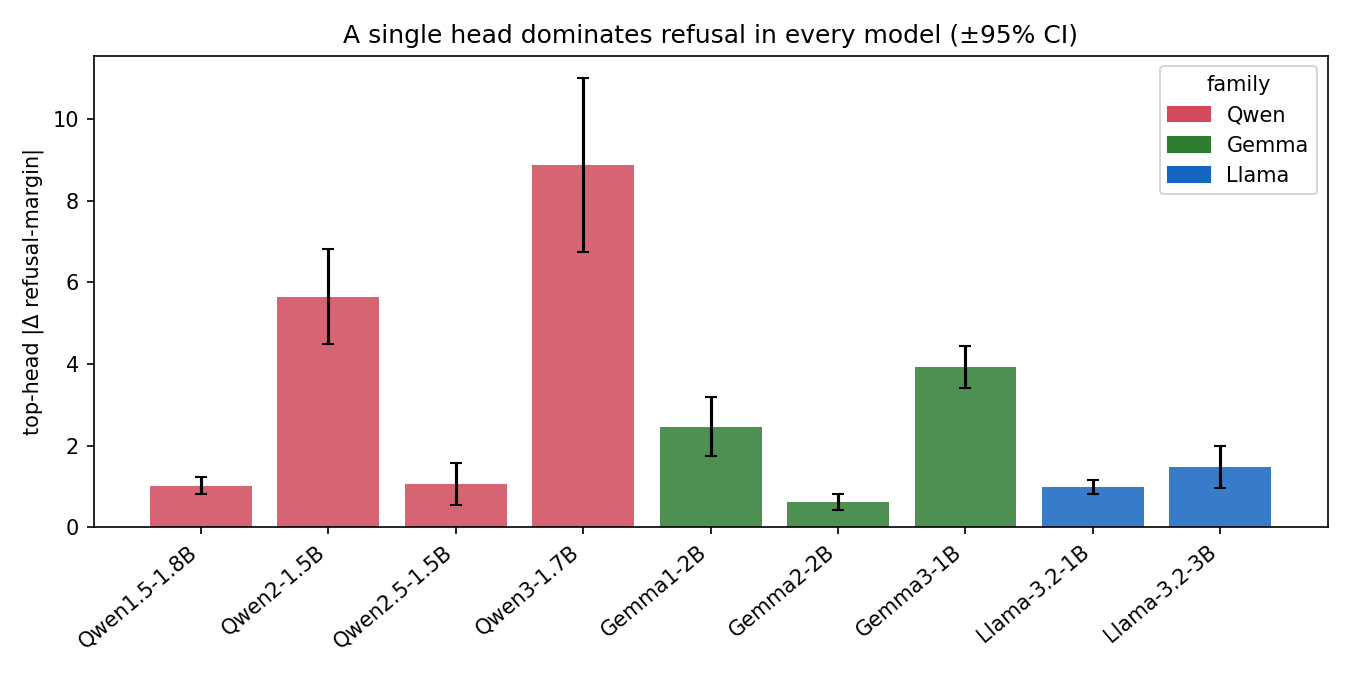
\includegraphics[width=\linewidth]{figures/fig_sparsity.png}
    \end{column}
    \begin{column}{0.38\textwidth}
      \footnotesize
      \begin{itemize}
        \item A single head dominates every model, well above its 95\% CI:\\
          \hl{Qwen3 L0H3 = 8.87 $\pm$ 2.13}.
        \item Patching one head benign$\rightarrow$harmful \emph{flips} the refusal logit --- \hl{causal, 9/9}.
        \item Heads \emph{cluster}, they are not scattered --- but \emph{where} they cluster varies by model (Finding C).
      \end{itemize}
    \end{column}
  \end{columns}
\end{frame}

% ---------------------------------------------------------------- 7. HEATMAPS
\begin{frame}{Where the safety heads sit}
  \framesubtitle{Per-head $|\Delta$ refusal-margin$|$ --- the patching map for all 9 models}
  \begin{columns}[c]
    \begin{column}{0.72\textwidth}
      \centering
      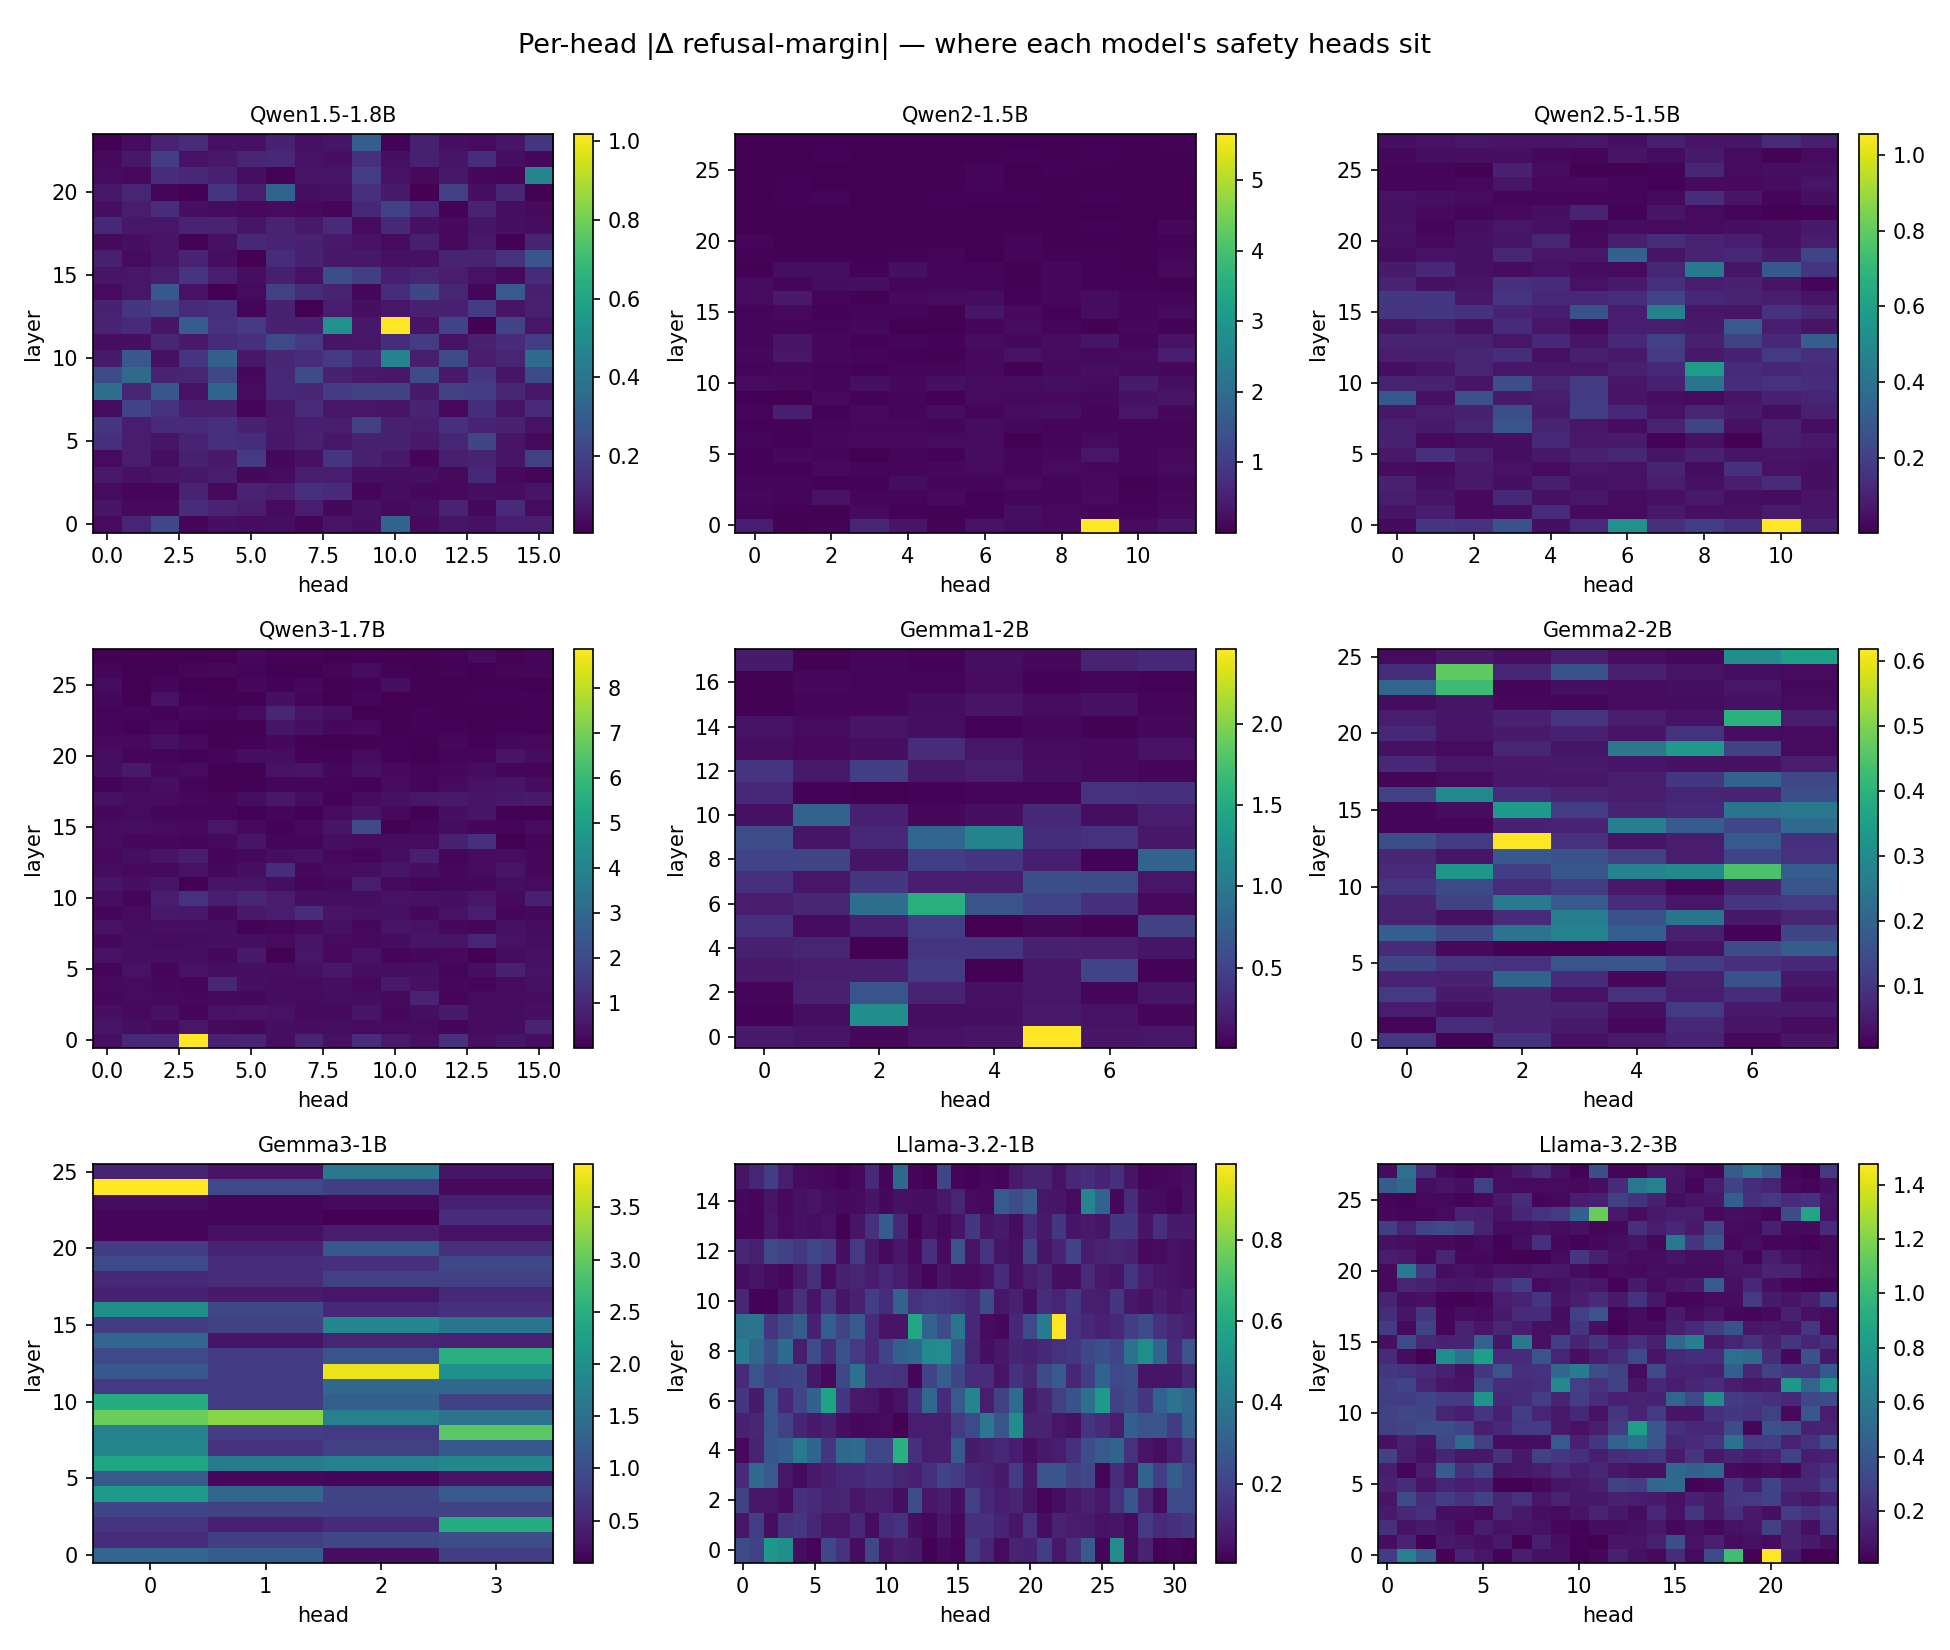
\includegraphics[height=0.74\textheight]{figures/fig_heatmaps.png}
    \end{column}
    \begin{column}{0.28\textwidth}
      \footnotesize
      \begin{itemize}
        \item One panel per model; axes are \hl{layer $\times$ head}, colour = causal importance.
        \item One or two \hlo{bright cells} stand out --- sparsity, seen directly.
        \item Their \emph{position} differs across models --- the seed of Finding~C.
      \end{itemize}
    \end{column}
  \end{columns}
\end{frame}

% ---------------------------------------------------------------- 8. FINDING A (HEADLINE)
\begin{frame}{Finding A --- concentrated, but not modular}
  \framesubtitle{The headline: removing refusal always breaks the model (H3b falsified)}
  \begin{columns}[c]
    \begin{column}{0.6\textwidth}
      \centering
      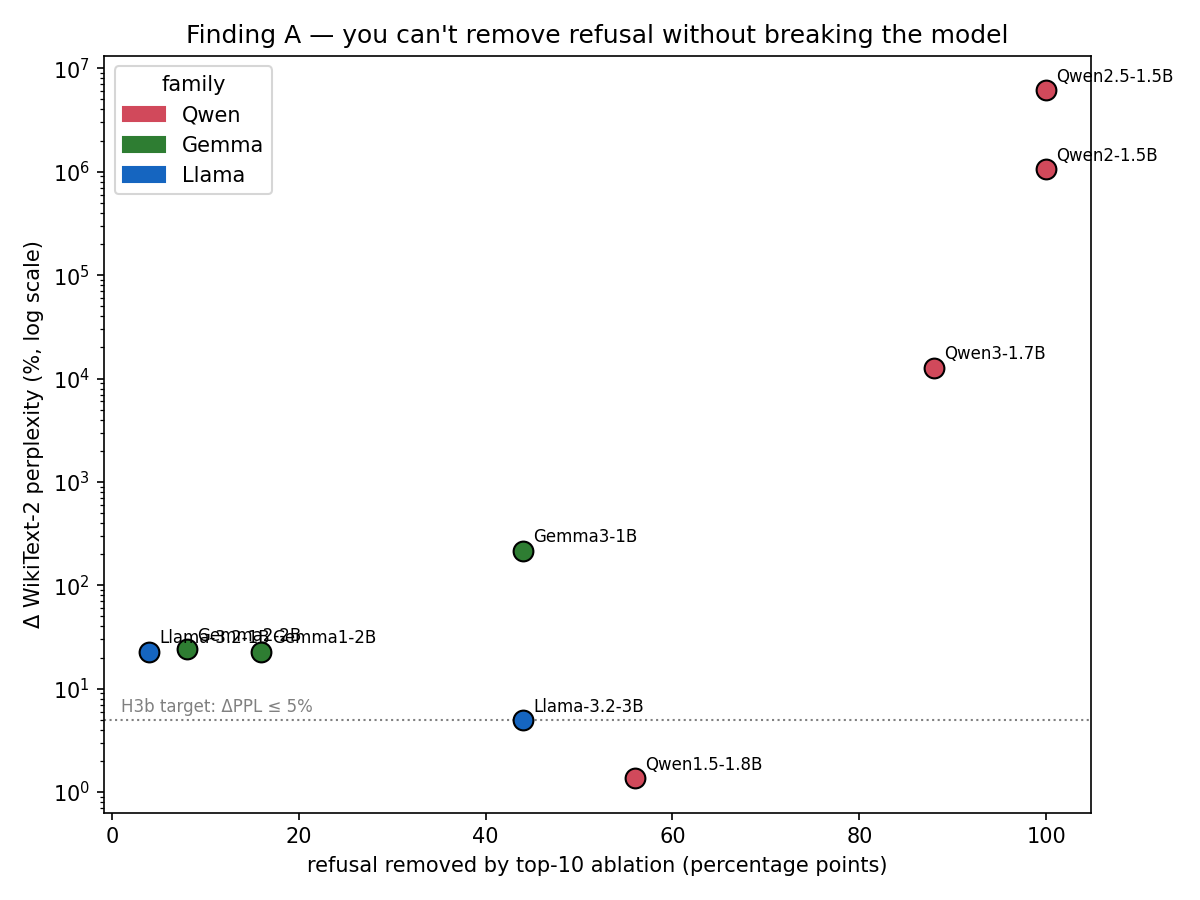
\includegraphics[width=\linewidth]{figures/fig_coupling.png}
    \end{column}
    \begin{column}{0.4\textwidth}
      \footnotesize
      \begin{itemize}
        \item The 4 models that drop to \hl{0\% refusal} are \emph{exactly} the 4 with the biggest perplexity blow-up.
        \item Qwen2.5: PPL \hlo{$\times$61{,}000}; output is \emph{gibberish}, not compliance.
        \item No model removes refusal \emph{and} keeps capability $\Rightarrow$ \hl{H3b falsified}.
        \item Refusal is entangled with the heads the model needs to generate coherent text.
      \end{itemize}
    \end{column}
  \end{columns}
\end{frame}

% ---------------------------------------------------------------- 8. FINDING B (DEPTH)
\begin{frame}{Finding B --- modularity scales with circuit \emph{depth}}
  \framesubtitle{Where the head sits decides how cleanly you can cut it}
  \begin{columns}[T]
    \begin{column}{0.5\textwidth}
      \textbf{Early (layer 0) $\Rightarrow$ catastrophic}
      \begin{itemize}
        \item Qwen top head at \hlo{L0}: zeroing it destroys coherence (PPL $\times$128 to $\times$61{,}000).
        \item These are general-purpose heads that \emph{also} gate refusal.
      \end{itemize}
    \end{column}
    \begin{column}{0.5\textwidth}
      \textbf{Late (layer 24) $\Rightarrow$ switch-like}
      \begin{itemize}
        \item \hl{Gemma-3-1B L24H0}: refusal $44\%\!\rightarrow\!0\%$ at only \hlo{+217\%} PPL.
        \item The \emph{only} model where ablation yields genuinely toxic output: \hl{RTP $\Delta$tox = +0.128} ($10\times$ any other).
      \end{itemize}
    \end{column}
  \end{columns}
  \vspace{4pt}
  \begin{block}{Takeaway}
    The cleanest, most ``switch-like'' safety circuit we find is \hl{late-layer}. Early-layer ``safety'' heads are really load-bearing generation heads.
  \end{block}
\end{frame}

% ---------------------------------------------------------------- 9. FINDING C (MIGRATION)
\begin{frame}{Finding C --- location migrates across generations}
  \framesubtitle{How a family implements refusal is a moving target}
  \begin{columns}[c]
    \begin{column}{0.6\textwidth}
      \centering
      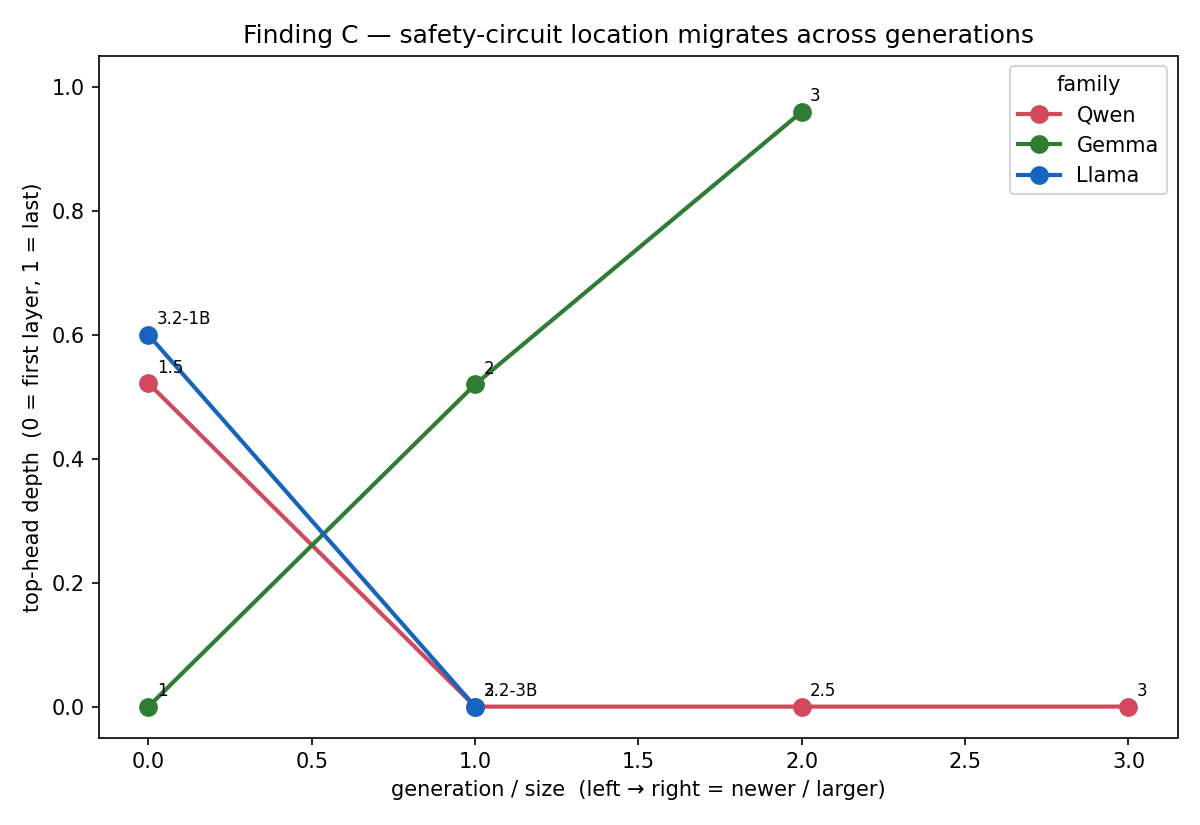
\includegraphics[width=\linewidth]{figures/fig_migration.png}
    \end{column}
    \begin{column}{0.4\textwidth}
      \footnotesize
      \begin{itemize}
        \item \hlo{Gemma} pushes safety \emph{deeper} each generation:\\ L0 $\rightarrow$ L13 $\rightarrow$ \hl{L24}.
        \item \hlo{Qwen} pulls it the \emph{other way}: mid-network (L12) $\rightarrow$ \hl{layer 0} from g2 on.
        \item \hlo{Llama-3B} is a \emph{hybrid}: early (L0) detection \emph{and} late (L24) enforcement.
        \item A novel within-family result --- refusal structure \hl{drifts across releases}.
      \end{itemize}
    \end{column}
  \end{columns}
\end{frame}

% ---------------------------------------------------------------- 10. FINDING D (JAILBREAK)
\begin{frame}{Finding D --- jailbreaks weaken refusal}
  \framesubtitle{Robustness is non-monotonic --- newer is not safer}
  \begin{columns}[c]
    \begin{column}{0.62\textwidth}
      \centering
      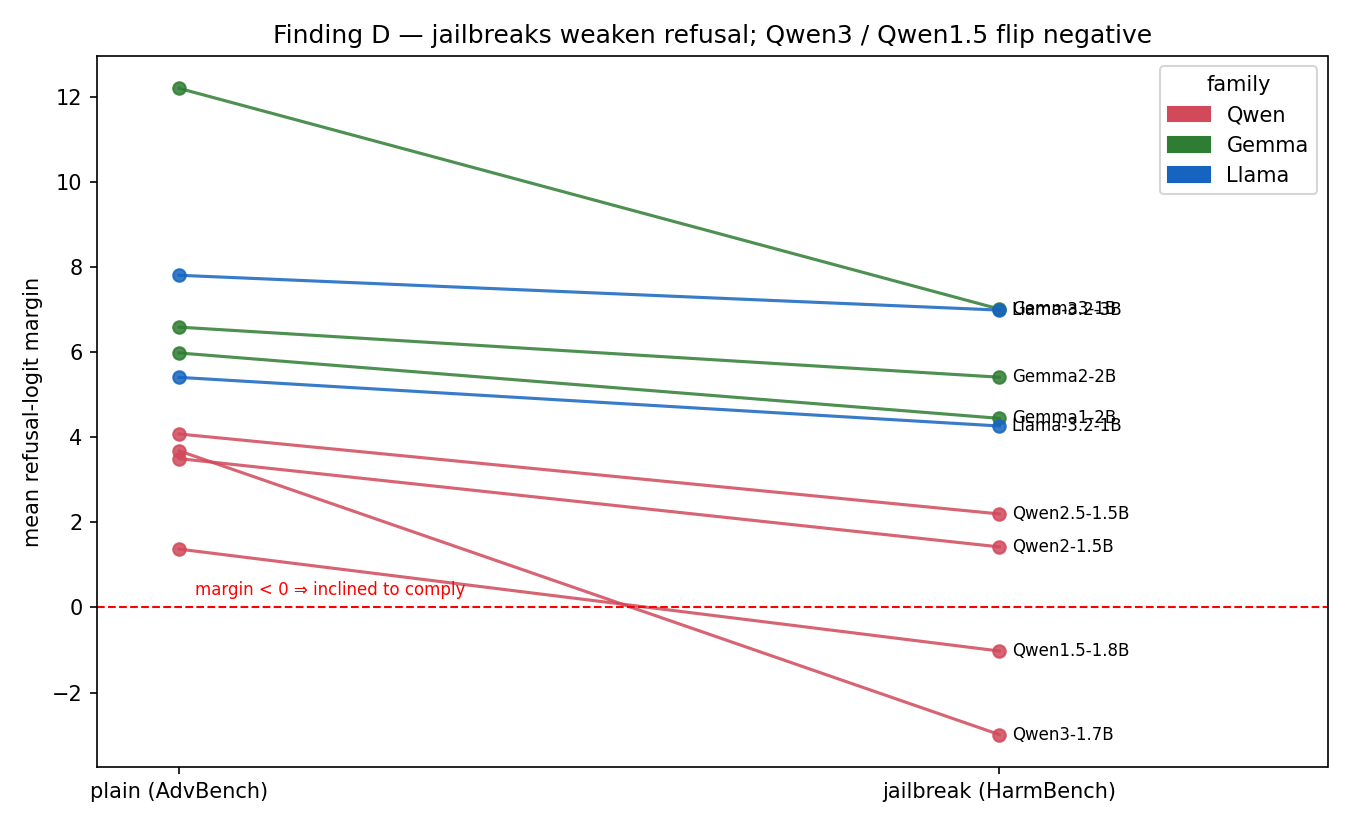
\includegraphics[width=\linewidth]{figures/fig_jailbreak.png}
    \end{column}
    \begin{column}{0.38\textwidth}
      \footnotesize
      \begin{itemize}
        \item Most robust: \hl{Gemma-2-2B} (96\%$\rightarrow$96\%, no drop); Llama-3B even rises (88\%$\rightarrow$96\%).
        \item Most brittle: \hl{Qwen3 \& Qwen1.5} --- refusal margin \emph{flips negative} under HarmBench (inclined to comply).
        \item \hlo{Qwen3 $<$ Qwen2.5}: the newest model is the most jailbreakable.
      \end{itemize}
    \end{column}
  \end{columns}
\end{frame}

% ---------------------------------------------------------------- 11. SCORECARD
\begin{frame}{Hypothesis scorecard}
  \framesubtitle{Sparse \& causal hold universally; ``clean removal'' does not}
  \small
  \renewcommand{\arraystretch}{1.3}
  \begin{tabular}{@{}c l c@{}}
    \toprule
    \textbf{H} & \textbf{Claim} & \textbf{Verdict} \\
    \midrule
    H1  & Sparse --- a dominant head + short tail                       & \good\ \textbf{holds 9/9} \\
    H2  & Causal --- patching flips the refusal logit                   & \good\ \textbf{confirmed 9/9} \\
    H3  & Ablation drives refusal $\le 30\%$                            & \pmark\ partial (5/9) \\
    H3b & \dots\ \emph{and} capability preserved ($\Delta$PPL $\le5\%$) & \bad\ \textbf{falsified} \\
    H4  & Same structure across models                                  & \pmark\ richer: location \emph{migrates} \\
    \bottomrule
  \end{tabular}
  \vspace{6pt}
  \begin{itemize}\footnotesize
    \item The pre-registered ``failure mode'' \emph{became} the contribution: refusal is \hl{concentrated but not modular}.
  \end{itemize}
\end{frame}

% ---------------------------------------------------------------- 13. FULL TABLE
\begin{frame}{Cross-model results at a glance (N = 50)}
  \framesubtitle{Top head · refusal removal · capability cost · jailbreak}
  \scriptsize
  \renewcommand{\arraystretch}{1.15}
  \setlength{\tabcolsep}{4pt}
  \begin{tabular}{@{}l c c c c c c@{}}
    \toprule
    \textbf{Model} & \textbf{L$\times$H} & \textbf{Top head} & \textbf{Refusal clean$\rightarrow$abl} & \textbf{$\Delta$PPL} & \textbf{JB refusal} & \textbf{Margin plain$\rightarrow$jb} \\
    \midrule
    Qwen1.5-1.8B  & 24$\times$16 & L12H10 & 80\%$\rightarrow$24\% & +1.4\%        & 80$\rightarrow$42 & $+1.37\rightarrow\mathbf{-1.02}$ \\
    Qwen2-1.5B    & 28$\times$12 & L0H9   & 100\%$\rightarrow$0\% & $\times$10{,}600 & 100$\rightarrow$74 & $+3.50\rightarrow+1.42$ \\
    Qwen2.5-1.5B  & 28$\times$12 & L0H10  & 100\%$\rightarrow$0\% & $\times$61{,}000 & 100$\rightarrow$94 & $+4.08\rightarrow+2.20$ \\
    Qwen3-1.7B    & 28$\times$16 & L0H3   & 88\%$\rightarrow$0\%  & $\times$128      & 88$\rightarrow$42 & $+3.68\rightarrow\mathbf{-2.99}$ \\
    Gemma1-2B     & 18$\times$8  & L0H5   & 88\%$\rightarrow$72\% & +23\%         & 88$\rightarrow$82 & $+5.98\rightarrow+4.44$ \\
    Gemma2-2B     & 26$\times$8  & L13H2  & 96\%$\rightarrow$88\% & +24\%         & \textbf{96$\rightarrow$96} & $+6.59\rightarrow+5.41$ \\
    Gemma3-1B     & 26$\times$4  & L24H0  & 44\%$\rightarrow$0\%  & +217\%        & 44$\rightarrow$36 & $+12.2\rightarrow+7.0$ \\
    Llama-3.2-1B  & 16$\times$32 & L9H22  & 96\%$\rightarrow$92\% & +23\%         & 96$\rightarrow$94 & $+5.41\rightarrow+4.26$ \\
    Llama-3.2-3B  & 28$\times$24 & L0H20  & 88\%$\rightarrow$44\% & +5\%          & 88$\rightarrow$96 & $+7.80\rightarrow+6.99$ \\
    \bottomrule
  \end{tabular}
  \vspace{4pt}\par
  \footnotesize
  Read Finding~A straight off the table: the four models at \hl{0\% refusal} are exactly the four with
  the biggest $\Delta$PPL. RTP $\Delta$toxicity is null everywhere except \hl{Gemma-3 (+0.128)}.
\end{frame}

% ---------------------------------------------------------------- 14. PATHS TO EXTEND
\begin{frame}{Where this goes next}
  \framesubtitle{From mapping the circuit to acting on it}
  \begin{columns}[T]
    \begin{column}{0.5\textwidth}
      \textbf{Make refusal modular}
      \begin{itemize}\footnotesize
        \item Steering vectors / refusal-direction edits \& weight surgery instead of blunt ablation.
        \item \hl{SAEs} to decompose the entangled L0 heads into separable features.
        \item Test the design lever directly: \emph{can a late-layer circuit be cut cleanly?}
      \end{itemize}
      \vspace{4pt}
      \textbf{Tighten rigor}
      \begin{itemize}\footnotesize
        \item Causal scrubbing; 50-prompt human metric audit; Llama-3B higher-K sweep.
      \end{itemize}
    \end{column}
    \begin{column}{0.5\textwidth}
      \textbf{Broaden coverage}
      \begin{itemize}\footnotesize
        \item Scale beyond 4B parameters --- does the picture hold at larger sizes?
        \item Multi-axis safety: deception, bias, PII --- not just toxicity.
        \item Cross-lingual refusal circuits.
        \item More model families, to test how general the depth$\rightarrow$modularity law is.
      \end{itemize}
    \end{column}
  \end{columns}
\end{frame}

% ---------------------------------------------------------------- 13. CONCLUSION
\begin{frame}{Conclusion}
  \framesubtitle{Safety is mechanistic --- but entangled}
  \begin{enumerate}
    \item Refusal is \hl{sparse and causal}: one dominant head, in all 9 models (H1/H2 \good).
    \item It is \hl{concentrated but not modular} --- removing it always costs capability (H3b \bad). \emph{Refusal-rate alone overstates a clean ``safety switch''.}
    \item \hl{Modularity scales with depth}; the circuit's \hl{location migrates} across generations; \hl{newer $\ne$ safer} under jailbreaks.
  \end{enumerate}
  \vspace{6pt}
  \begin{block}{Methodological lesson}
    A \hl{capability control} (perplexity) is mandatory in any ablation study --- without it, ``refusal $\rightarrow$ 0\%'' reads as success when it is really model breakage.
  \end{block}
  \vspace{4pt}
  \centering\small Thank you --- questions welcome.
\end{frame}

\end{document}
